\chapter{Methodology} \label{chap:methodology}
Many computer vision applications such as 3D object reconstruction or visual SLAM require the depth information from RGBD cameras. 
However, the results of these applications are often not unsatisfying because of the low quality of the depth acquisition from the cheap cameras. 
It would be gratifying if we can improve the depth quality without changing to an expensive camera.
Therefore, the depth refinement techniques play an essential role here.

In this chapter, we first introduce some pre-processing techniques to fill the missing areas and reduce the noise of the input depth image. 
Then, we describe in detail one of the state-of-the-art depth refinement method from Or-El \emph{et al.}~\cite{or2015rgbd} which we have chosen to implement as a starting point.
A proposed method based on a RGB ratio model is then followed and introduced to eliminate the nonlinearity in most of modern depth enhancement method.
Finally, another proposed technique which does not require any regularization terms is presented. 
This method has also exhibited the ability of dealing with the objects with complicated albedos and extension to depth super-resolution.
 

%%%%%%%%%%%%%%%%%%%%%%%%%%%%%%%%%%%%%%%%%%%%
\section{Pre-Processing}
%%%%%%%%%%%%%%%%%%%%%%%%%%%%%%%%%%%%%%%%%%%%
The first step for most of the image processing tasks is to pre-process the initial input image. 
Due to the hardware limitation of modern inexpensive RGBD sensors, there usually exist holes with missing values on the depth images. 
Also, the depth data is often noisy so we need to do denoising and acquire a relative smooth surface.

In this section, we will describe respectively the basic depth inpainting and denoising algorithm that we use for our pre-processing. 
%----------------------------------------------
\subsection{Depth inpainting}
%----------------------------------------------

%\begin{figure}[!htbp]
% \centering
% 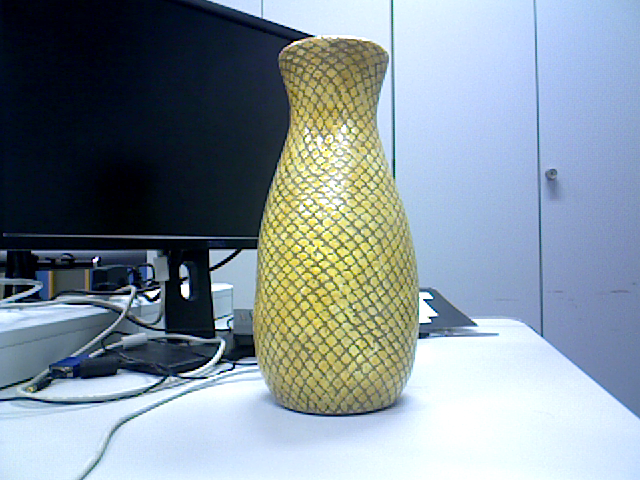
\includegraphics[width=0.45\textwidth]{figures/methodology/inpainting_rgb.png}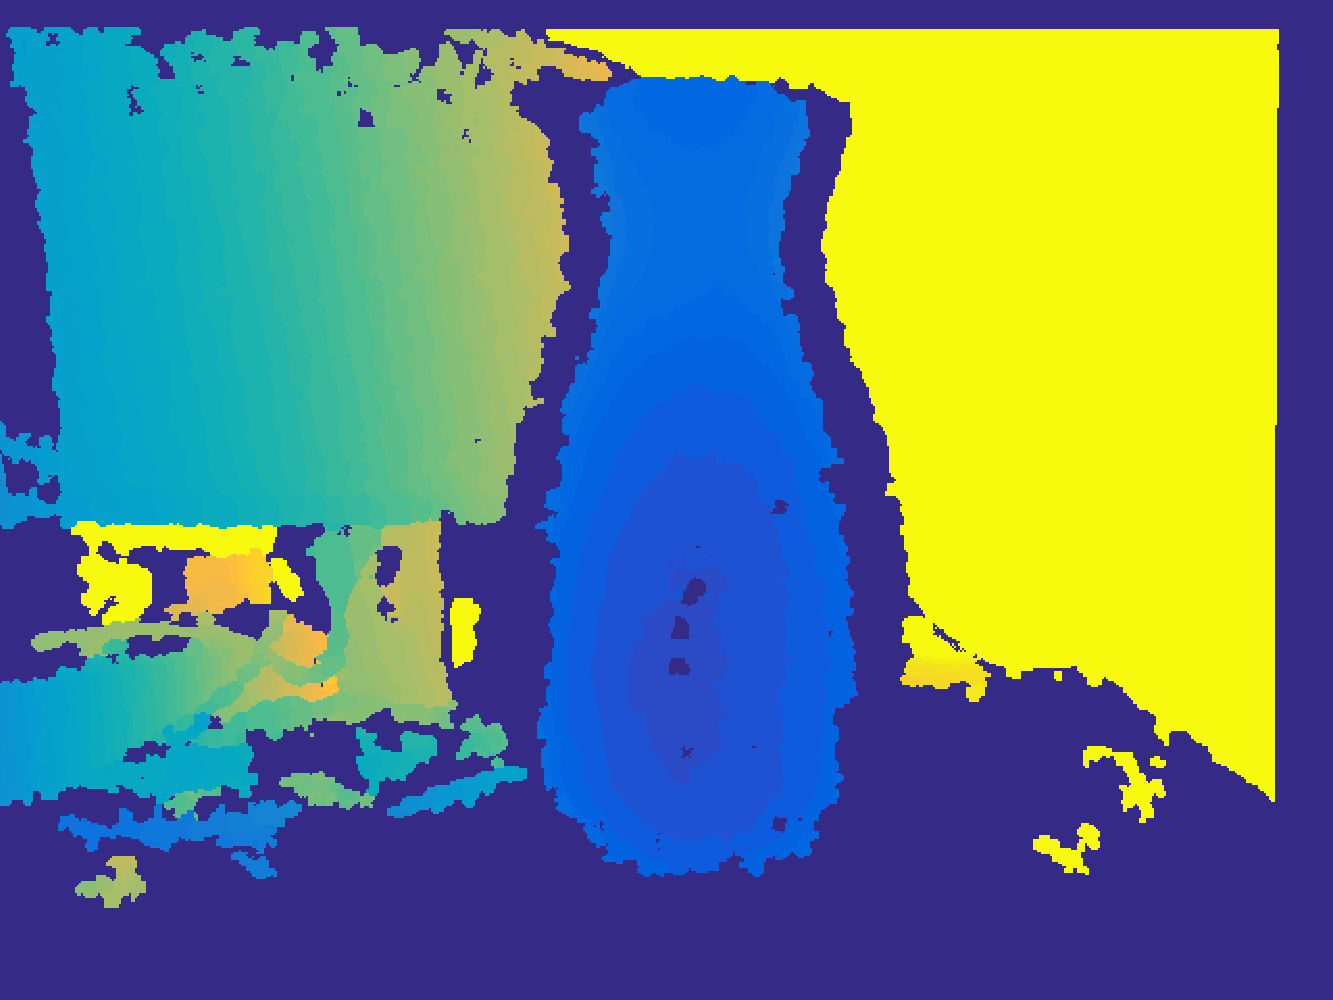
\includegraphics[width=0.45\textwidth]{figures/methodology/inpainting_depth.pdf}
% \caption{dd}
% \label{fig:inpainting1}
%\end{figure}

Image inpainting itself is a very mutual area and has been widely applied as a useful tool for many modern computer vision applications, e.g, restore the damaged parts of ancient paintings, or remove unwanted texts or objects in a photography~\cite{bertalmio2000image}. 
Since the idea of image inpainting is to automatically replace the lost or undesired parts of an image with the neighbouring information by interpolating, we were inspired to apply it to fill in the missing depth information (Fig.~\ref{fig:inpainting1}).

\begin{figure}[!htbp]
\centering
\subfigure[RGB image]{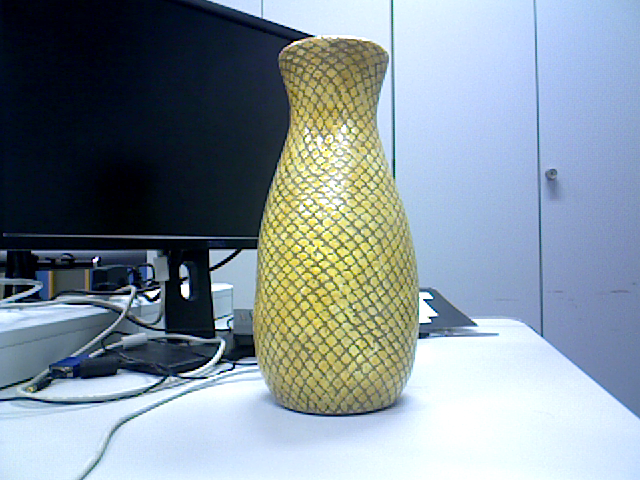
\includegraphics[width=0.45\linewidth]{figures/methodology/inpainting_rgb.png}}
\subfigure[Input depth image]{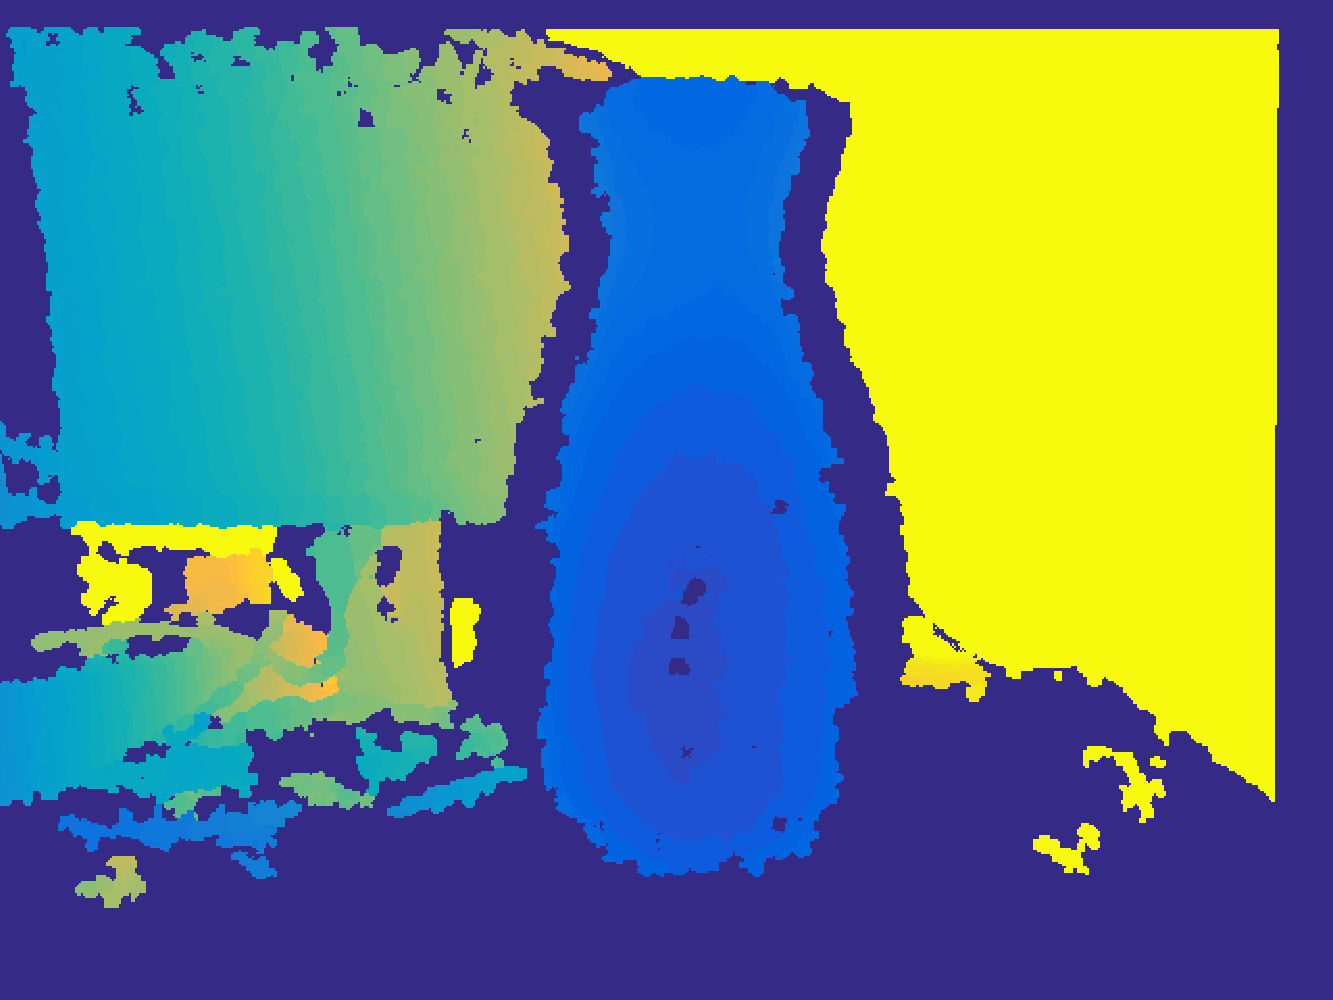
\includegraphics[width=0.45\linewidth]{figures/methodology/inpainting_depth.pdf}}
\caption{The input RGB and depth image of a vase. The brighter color on the image (b), the higher depth values.}
\label{fig:inpainting1}
\end{figure}

It should be noted that, the depth inpainting is applied to the input noisy image so there is no need to use some powerful and advanced algorithms.
The only request is to fill the missing areas with inexpensive computational time.

The general mathematical form of a classic inpainting algorithm~\cite{bertalmio2000image} can be written as follows

\begin{equation}\label{eq:method_inpaint1}
I^{t+1}(i,j) = I^{t}(i,j) + \mu U^{t}(i,j), \forall(i,j)\in \Omega
\end{equation}
where $I(i,j)$ is the pixel value in image $I$, $t$ is the artificial time step, $\mu$ is the updating rate, $U$ is the update information and $\Omega$ are the area with missing information.

To build the update map $U$ in each time step, there are two principles that~\cite{bertalmio2000image} follow.
One is the inpainted values inside $\Omega$ should be as smooth as possible. 
The other is the lines reaching the edge of $\Omega$ should be continued and cross the missing area, while the values in $\Omega$ should be propagated from the nearest neighbours of $\Omega$ along the lines.

Again, due to the fact that our input depth images have poor quality, the lines arriving at the boundary $\delta \Omega$ may be incorrect or produced by the noises.
Thus, it is reasonable that our initial depth inpainting problem focuses on the smooth propagation from the neighbours and fill in the holes.

In each pixel $(x_0, y_0)$ inside $\Omega$, $U$ can be modelled as a discrete four-neighbour Laplacian operator:
\begin{equation}
\begin{split}
U(x_0, y_0) = \Delta I
		        = 4I(x_0, y_0) - I(x_0 + 1, y_0) - I(x_0 - 1, y_0) - I(x_0, y_0+1) - I(x_0 , y_0 -1)
\end{split}
\end{equation}
Now the inpainting problem in Eq.~\ref{eq:method_inpaint1} can be represented as a minimization problem: 
\begin{equation}
\min \iint\limits_{\Omega} |U(x,y)|^2 dxdy 
\end{equation}
This problem can be reformulated to a typical linear equation in matrix form:
\begin{equation}
\mathbf{Ax=b}
\end{equation}
Assuming $n$ is the number of pixel inside $\Omega$ and $m$ is the sum of $n$ and the number of neighbouring pixel around the boundary $\delta \Omega$, $\mathbf{A}$ is a $m\times n$ Laplacian matrix, $\mathbf{b}$ is a $m\times1$ vector containing all the known boundary depth values and the $0$ inside $\Omega$.
Solving the linear equation with simple least square method, we can acquire the inpainted values.
With our this naive image inpainting algorithm, we can fill the holes on the depth image as shown in Fig.~\ref{fig:pre-processing}.

%----------------------------------------------
\subsection{Depth denoising}
%----------------------------------------------
the depth images acquired from the RGB-D cameras with moderate price usually contain various noises. 
As a standard pre-processing method, the image denoising technique is also applied to our input inpainted depth map.
Similar to the state-of-the-art depth refinement methods~\cite{zhang2012edge, or2015rgbd, han2013high, or2016real, haque2014high, yu2013shading}, bilateral fitering~\cite{tomasi1998bilateral} is used as our depth pre-processing smoother. 

The advantages of bilateral filter is reducing the noise while preserving the edge in the input image. 
More than a regular Gaussian smooth filter, which uses only the difference of the image values (depth in our case) between the center pixel the neighbours, the bilateral filter also utilizes the space difference as a reference to build up the weighting function.
The filtered pixel value can be modelled as a weighted sum of neighbouring pixels:
\begin{equation}
\hat{I}(\mathbf{x}) = \frac{1}{W}\sum_{\mathbf{y} \in \mathcal{N}} I(\mathbf{y})e^{-(\frac{\lVert I(\mathbf{x}) - I(\mathbf{y})\rVert^2}{2\sigma_r^2} + \frac{\lVert \mathbf{x} - \mathbf{y}\rVert^2}{2\sigma_d^2})}
\end{equation}
where $\hat{I}(\mathbf{x})$ is the filtered value at pixel $\mathbf{x}$, $\mathcal{N}$ represents the neighbouring pixels with $\mathbf{x}$ in the center, and $W$ is the the sum of the all the weights. 
The smoothed result on our input depth image is shown in Fig.~\ref{fig:pre-processing}.

\begin{figure}[!htbp]
\centering
\subfigure[Input depth]{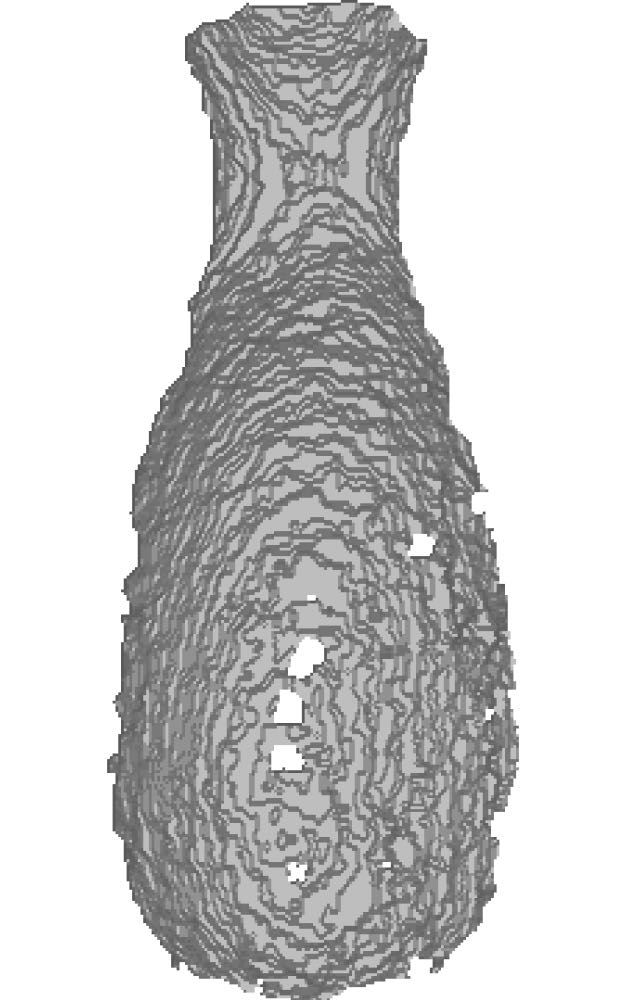
\includegraphics[width=0.30\linewidth]{figures/methodology/inpainting_shape_before.pdf}}
\subfigure[After inpainting]{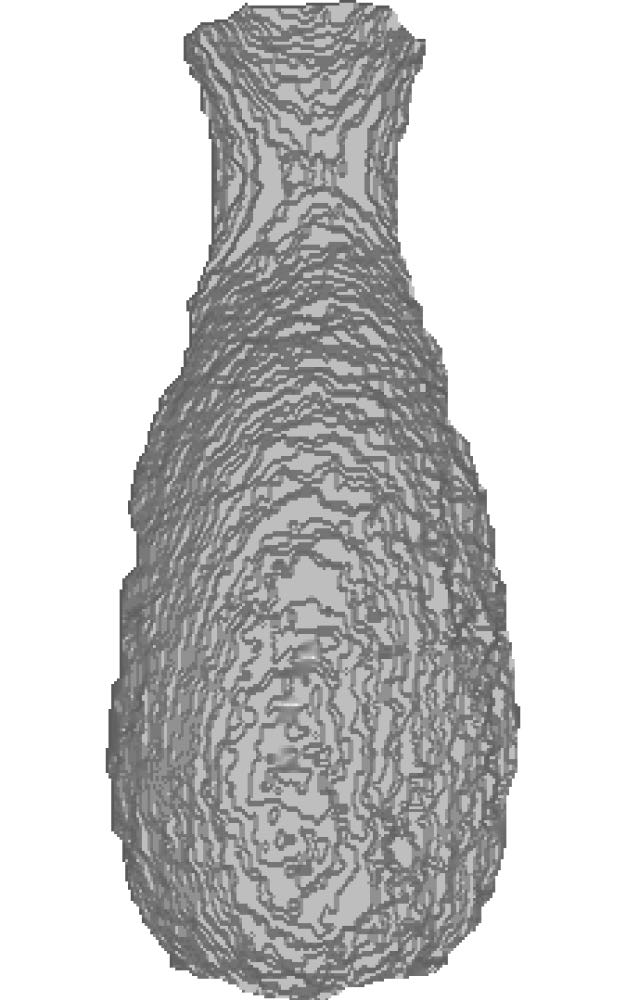
\includegraphics[width=0.30\linewidth]{figures/methodology/inpainting_shape_after.pdf}}
\subfigure[After smoothing]{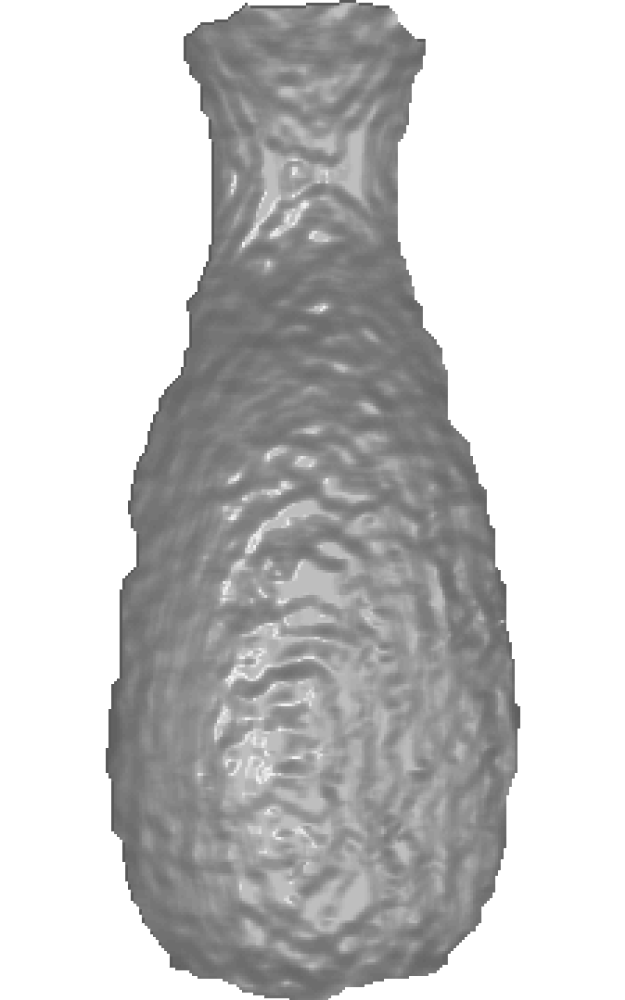
\includegraphics[width=0.30\linewidth]{figures/methodology/smooth_shape_after.pdf}}
\caption{Illustrations for the pre-processing on the depth of the vase.}
\label{fig:pre-processing}
\end{figure}

After the pre-processing procedure, we have an initial smooth and inpainted depth image. 
It will be used as the input of all the depth refinement methods detailed in the following sections.

%%%%%%%%%%%%%%%%%%%%%%%%%%%%%%%%%%%%%%%%%%%%
\section{RGBD-Fusion method}
%%%%%%%%%%%%%%%%%%%%%%%%%%%%%%%%%%%%%%%%%%%%
RGBD-Fusion is a state-of-the-art depth recovery method proposed by Or-El \emph{et al.}~\cite{or2015rgbd}.
This novel method is adequate for natural scene illumination and able to enhance the depth map much faster than other methods.
It is reasonable to gain a comprehensive understanding in the field of depth refinement by implementing this method.

It is worth mentioning that we didn't just follow the paper step by step without injecting any our own ideas.
For example, instead of estimating the pixel-wise ambient light with a separate energy function, we jointly calculated all four first-order spherical harmonics parameters (3 for point-source light direction and 1 for ambient light) with a simple fast least square, and the results have only negligible difference.
And throughout the whole estimation process of light, albedo and depth, we only used the information within the given mask which also speeded up the algorithm.

In the following part of this section, we will explain the method and more our implementation details can be found in Appendix~\ref{appendix:implement}.

%----------------------------------------------
\subsection{Light estimation}
%----------------------------------------------
The natural uncalibrated illumination condition means the light is no longer a point light source, thus a Lambertian model is not sufficient. 
Basri and Jocobs~\cite{basri2003lambertian} has found that low order spherical harmonics (SH) model can well set out the irradiance of the diffused objects under the natural scene.
More specifically, the first-order SH model can capture 87.5\% of natural lighting, whose form is extended from the Lambertian model:
\begin{equation}\label{eq:rgbd_light_model}
I(x,y) = \rho(x,y)(\mathbf{l}^\top \mathbf{n} + \varphi)
\end{equation}
where $I$ is the irradiance of the objects, which is represented as the intensity values, $\rho$ is the albedo, $\mathbf{l}^\top = \begin{pmatrix} l_x & l_y & l_z \end{pmatrix}$ describes the light direction and $\varphi$ represents the ambient light.
Here the surface normal $\mathbf{n}$ is formulated with orthographic projection, i.e. 
\begin{equation}
	\mathbf{n} = \frac{1}{\sqrt{1 + |\nabla z|^2}}
	\begin{pmatrix} 
		 \nabla z\\ 
		 -1
	 \end{pmatrix}
\end{equation}
$\nabla z$ represents the gradient of depth image $z(x,y)$ in $x$ and $y$ directions.
Since we have the input depth from pre-processing, initial $\mathbf{n}_0$ is known.

In the sense of intrinsic image decomposition, an image can be decomposed as the product of albedo and shading, so we can treat $\mathbf{l}^\top \mathbf{n} + \varphi$ in Eq.~\ref{eq:rgbd_light_model} as the shading $S(x,y)$.
Therefore, we have:
\begin{equation}
S(x,y) = \mathbf{l}^\top \mathbf{n} + \varphi = \mathbf{s} \boldsymbol{\cdot} \tilde{\mathbf{n}}
\end{equation}
where
\begin{equation}
\mathbf{s} = \begin{pmatrix}\mathbf{l} \\ \varphi \end{pmatrix}   \; \; \tilde{\mathbf{n}} = \begin{pmatrix}\mathbf{n} \\ 1\end{pmatrix}  
\end{equation}
To compute the spherical harmonics parameters, we assume the albedo $\rho$ equals to $1$ for each pixel. 
Since there are known intensity value and surface normal in each pixel within the mask, we will have an overdetermined least square problem: 
\begin{equation}
\argmin_{\mathbf{s}} \lVert I - \mathbf{s} \boldsymbol{\cdot} \tilde{\mathbf{n}} \rVert^2_2
\end{equation}
This process only need to be applied once at the beginning of the process since the least squares is not sensitive to the details on the surface, thus the estimation from the smooth surface is enough.

%----------------------------------------------
\subsection{Albedo estimation}
%----------------------------------------------
In order to acquire the a satisfying depth refinement outcome, an effective albedo estimation process is a matter of importance.
If no regularization is imposed, the albedo image can be directly obtained from $I/S$, which is usually susceptible because of overfitting. 
Therefore, a prior that emphasizes the piecewise smoothness on the albedo is applied.

%----------------------------------------------
\subsection{Depth enhancement}
%----------------------------------------------

%%%%%%%%%%%%%%%%%%%%%%%%%%%%%%%%%%%%%%%%%%%%
\section{Proposed method I: RGB Ratio Model}
%%%%%%%%%%%%%%%%%%%%%%%%%%%%%%%%%%%%%%%%%%%%



%----------------------------------------------
\subsection{Limitations}
\begin{itemize}
\item \emph{LEDs have to be set up far away from each other.}
\item \emph{Natural illumination is a problem.}
\item \emph{Only feasible for the simple albedo cases}
\item \emph{Non specular objects}
\end{itemize}
%----------------------------------------------


%%%%%%%%%%%%%%%%%%%%%%%%%%%%%%%%%%%%%%%%%%%%
\section{Proposed method II: Robust Lighting Variation Model without Regularization}

%----------------------------------------------
\subsection{Depth super-resolution}
%----------------------------------------------


%%%%%%%%%%%%%%%%%%%%%%%%%%%%%%%%%%%%%%%%%%%%

